\documentclass{article}

\usepackage{Sweave}
\begin{document}
\Sconcordance{concordance:APBTestBasics.tex:APBTestBasics.Rnw:%
1 2 1 1 0 2 1 1 2 1 0 1 1 4 0 2 2 1 0 2 1 4 0 1 2 1 1 1 2 1 0 1 1 9 0 1 %
2 3 1 1 4 2 1}


\begin{Schunk}
\begin{Sinput}
> x <- rnorm(100)
> hist(x)
\end{Sinput}
\end{Schunk}
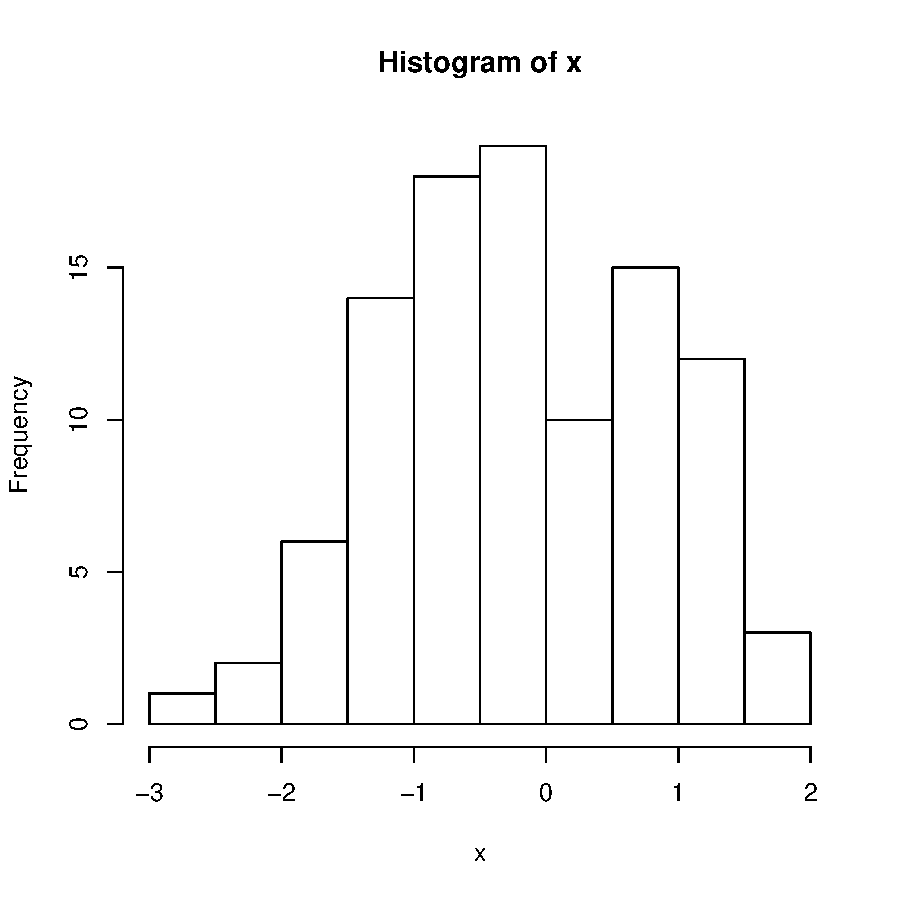
\includegraphics{APBTestBasics-C1}

\begin{Schunk}
\begin{Sinput}
> x <- rnorm(100)
> y <- rnorm(100)
> plot(x,y)
\end{Sinput}
\end{Schunk}
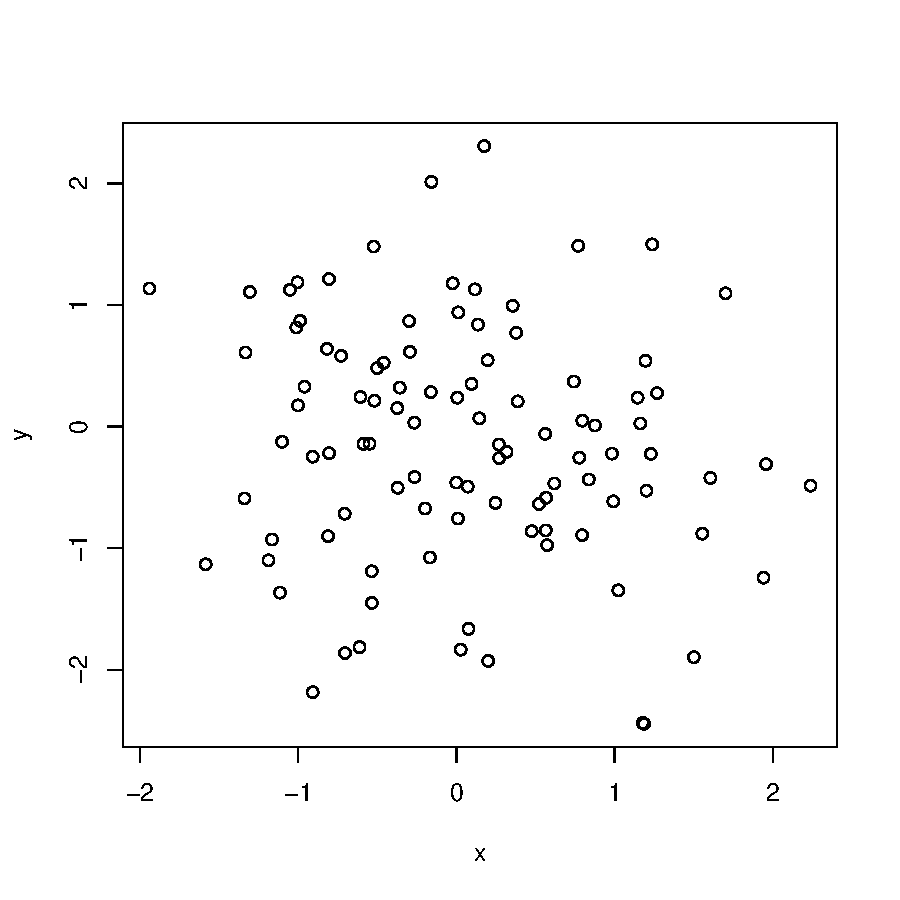
\includegraphics{APBTestBasics-examplePlot}


\begin{Schunk}
\begin{Sinput}
> data(airquality)
> kruskal.test(Ozone ~ Month, data = airquality)
\end{Sinput}
\begin{Soutput}
	Kruskal-Wallis rank sum test

data:  Ozone by Month
Kruskal-Wallis chi-squared = 29.267, df = 4, p-value = 6.901e-06
\end{Soutput}
\end{Schunk}
which shows that the location parameter of the Ozone 
distribution varies significantly from month to month. Finally we
include a boxplot of the data:



\end{document}
